\newpage
\def\thoigian{90}%--Thời gian
\de{Đề số 3}{Chương IX. Phương pháp tọa độ trong mặt phẳng}


\begin{center}
	\textbf{PHẦN 1-CÂU TRẮC NGHIỆM BỐN PHƯƠNG ÁN}
\end{center}
\Opensolutionfile{ans}[ans/ans-TN-ONTAPCHUONG-DE1]
%Câu 1
\begin{ex}%[Dự án D đợt 3, Thanh Phong]%[0H9N1-1]
		Trong mặt phẳng $Oxy$, cho hai điểm $A(-3;1)$ và $B(1;2)$. Độ dài vectơ $\overrightarrow{AB}$ bằng 
		\choice
		{$17$}
		{$\sqrt{5}$}
		{\True $\sqrt{17}$}
		{$5$}
		\loigiai{
			Ta có $\overrightarrow{AB}=\left(4;1\right) \Rightarrow \left| \overrightarrow{AB}\right| =AB=\sqrt{4^2+1^2}=\sqrt{17}$.
		}
\end{ex}
%Câu 2
\begin{ex}%[Dự án D đợt 3, Thanh Phong]%[0H9N1-4]
	Trong mặt phẳng tọa độ $Oxy$, cho hai vectơ $\overrightarrow{a}=(1;\sqrt{3})$ và $\overrightarrow{b}=(1;0)$. Tính góc $\alpha$ giữa hai vectơ $\overrightarrow{a}$ và $\overrightarrow{b}$.
	\choice
	{$\alpha=135^\circ$}
	{$\alpha=30^\circ$}
	{$\alpha=45^\circ$}
	{\True $\alpha=60^\circ$}
	\loigiai{
		Ta có $\cos\alpha=\dfrac{\overrightarrow{a}\cdot\overrightarrow{b}}{\left|\overrightarrow{a}\right|\cdot\left|\overrightarrow{b}\right|}=\dfrac{1\cdot 1+\sqrt{3}\cdot 0}{\sqrt{1^2+(\sqrt{3})^2}\cdot\sqrt{1^2+0^2}}=\dfrac{1}{2}$.\\
		Vậy góc tạo bởi hai vectơ $\overrightarrow{a}$ và $\overrightarrow{b}$ là $\alpha=60^\circ$.
	}
\end{ex}
%Câu 3
\begin{ex}%[Dự án D đợt 3, Thanh Phong]
	Trong mặt phẳng với hệ tọa độ $Oxy$, cho hai điểm $A(-2;3)$, $B(2;5)$. Tọa độ trung điểm của đoạn $BA$ là 
	\choice
	{\True $(0;4)$}
	{$(-1;2)$}
	{$(0;2)$}
	{$(2;-1)$}
	\loigiai{
		Gọi $M$ là trung điểm $BA$, ta có $\heva{&x_M=\dfrac{x_A+x_B}{2}=\dfrac{-2+2}{2}=0\\&y_M=\dfrac{y_A+y_B}{2}=\dfrac{3+5}{2}=4.}$\\
		Vậy $M(0;4)$.
	}
\end{ex}
%Câu 4
\begin{ex}%[Dự án D đợt 3, Thanh Phong]%[0H9H1-1]
	Cho tam giác $ABC$ có tọa độ các đỉnh $A(-8;0)$, $B(0;6)$, $C(2;0)$. Chu vi $\triangle ABC$ là
	\choice
	{$10+2\sqrt{10}$}
	{$20-2\sqrt{10}$}
	{\True $20+2\sqrt{10}$}
	{$10-2\sqrt{10}$}
	\loigiai{
		Ta có $AB=\sqrt{8^2+6^2}=10$; $AC=\sqrt{(2+8)^2+0^2}=10$; $BC=\sqrt{2^2+(-6)^2}=2\sqrt{10}$.\\
		Từ đó chu vi $\triangle ABC$ là  $AB+AC+BC=20+2\sqrt{10}$.}                               
\end{ex}
%Câu 5
\begin{ex}%[Dự án D đợt 3, Thanh Phong]%
	Trong mặt phẳng $Oxy$, cho dường thẳng $(d)$ có phương trình tham số $\heva{&x=-5+2t\\&y=2+t}$, $t\in \mathbb{R}$. Tìm tọa độ điểm $M$ thuộc $(d)$ biết hoành độ của điểm $M$ là $-7$.
	\choice
	{\True $M(-7;1)$}
	{$M(-23;-7)$}
	{$M(-7;-19)$}
	{$M(1;-7)$}
	\loigiai{
		Ta có $x_M = -7 \Rightarrow -7 = -5 + 2t \Leftrightarrow t = -1$.\\
		Với $t = -1 \Rightarrow y_M = 1$. Vậy $M(-7;1)$.
	}
\end{ex}
%Câu 6
\begin{ex}%[Dự án D đợt 3, Thanh Phong]%
	Cho đường thẳng $\Delta \colon 3x-4y+1=0$. Tính khoảng cách từ điểm $M(2;3)$ đến đường thẳng $\Delta$.
	\choice
	{\True $1$}
	{$\dfrac{6}{5}$}
	{$2$}
	{$\sqrt{5}$}
	\loigiai{
		Ta có khoảng cách từ điểm $M(2;3)$ đến đường thẳng $\Delta$ là $\mathrm{d}\left(M, \Delta \right)=\dfrac{|3 \cdot 2-4 \cdot 3+1|}{\sqrt{3^2+4^2}}=\dfrac{5}{5}=1$.}
\end{ex}
%Câu 7
\begin{ex}%[Dự án D đợt 3, Thanh Phong]%
	Tìm điều kiện của tham số $m$ để phương trình $x^2+y^2-2x+4y-m=0$ là phương trình của một đường tròn.
	\choice
	{$m>5$}
	{$m \ge -5$}
	{$-5<m<5$}
	{\True $m > -5$}
	\loigiai{
		Để phương trình $x^2+y^2-2x+4y-m=0$ là phương trình của một đường tròn thì
		$$1^2+(-2)^2+m>0\Leftrightarrow m>-5.$$
	}	
\end{ex}
%Câu 8
\begin{ex}%[Dự án D đợt 3, Thanh Phong]%
	Trong mặt phẳng tọa độ $Oxy$, đường tròn có đường kính $AB$ với $A(0; 3)$ và $B(-2; 5)$ có phương trình là 
	\choice
	{\True $(x+1)^2+(y-4)^2=2$}
	{$(x-1)^2+(y+4)^2=8$}
	{$(x+1)^2+(y-4)^2=8$}
	{$(x-1)^2+(y+4)^2=2$}
	\loigiai{
		Gọi $I(x_I,y_I)$ là trung điểm của $AB$. Khi đó \allowdisplaybreaks
		\begin{eqnarray*}
			\heva{& x_I=\dfrac{x_A+x_B}{2} \\ & y_I=\dfrac{y_A+y_B}{2}} \Rightarrow\heva{& x_I=\dfrac{0+(-2)}{2}=-1 \\ & y_I=\dfrac{3+5}{2}=4} \Rightarrow I(-1; 4).
		\end{eqnarray*}
		Ta có $AB=\sqrt{(-2-0)^2+(5-3)^2}=2 \sqrt{2}$.\\
		Đường tròn đường kính $AB$ có tâm $I(-1; 4)$ bán kính $R=\dfrac{A B}{2}=\dfrac{2 \sqrt{2}}{2}=\sqrt{2}$ nên có phương trình
		\allowdisplaybreaks
		\begin{eqnarray*}
			(x+1)^2+(y-4)^2=(\sqrt{2})^2 \Leftrightarrow(x+1)^2+(y-4)^2=2.
		\end{eqnarray*}
		
	}
\end{ex}
%Câu 9
\begin{ex}%[Dự án D đợt 3, Thanh Phong]%
	Trong mặt phẳng với hệ tọa độ $Oxy$, cho hai điểm $A(-2;3)$, $B(0;1)$. Gọi $(T)$ là tập hợp điểm $M$ thỏa mãn $\overrightarrow{MA}\cdot\overrightarrow{MB}=0$. Tính diện tích $S$ phần hình phẳng giới hạn bởi $(T)$.
	\choice
	{$S=2\sqrt{2}\pi$}
	{$S=\sqrt{2}\pi$}
	{\True $S=2\pi$}
	{$S=4\pi$}
	\loigiai{
		Vì $\overrightarrow{MA}\cdot\overrightarrow{MB}=0\Rightarrow MA\perp MB\Rightarrow \widehat{AMB}=90^{\circ}\Rightarrow M$ nằm trên đường tròn đường kính $ AB $.\\
		Mà $ AB=\sqrt{4+4}=2\sqrt{2}\Rightarrow $ bán kính $ R=\sqrt{2} $.\\
		Do vậy, diện tích $ S=\pi (\sqrt{2})^{2}=2\pi $.
	}
\end{ex}
%Câu 10
\begin{ex}%[Dự án D đợt 3, Thanh Phong]%
	Trong mặt phẳng $Oxy$, cho elip $(E)\colon \dfrac{x^2}{16}+\dfrac{y^2}{9}=1$. Tính độ dài trục lớn của $(E)$.
	\choice
	{$9$}
	{$6$}
	{$16$}
	{\True $8$}
	\loigiai{
		Theo giả thiết $a=4$. Độ dài trục lớn của $(E)$ là $2a=8$.
	}
\end{ex}
%Câu 11
\begin{ex}%[Dự án D đợt 3, Thanh Phong]%
	Trong mặt phẳng $(Oxy)$, nếu hypebol có phương trình $\dfrac{x^2}{16}-\dfrac{y^2}{9}=1$ thì tiêu cự của nó là
	\choice
	{$4$}
	{$5$}
	{$20$}
	{\True $10$}
	\loigiai{Ta có $\heva{&a^2=16\\&b^2=9} \Leftrightarrow \heva{&a=4\\&b=3.}$\\
		Mà $c=\sqrt{a^2+b^2} \Leftrightarrow c=5$.\\
		Tiêu cự $F_1F_2=2c=10$.
	}
\end{ex}
%Câu 12
\begin{ex}%[Dự án D đợt 3, Thanh Phong]%
	Trong mặt phẳng tọa độ $Oxy$, cho parabol $(P)$ có phương trình $y^2=8 x$. Phương trình đường chuẩn của parabol là
	\choice
	{\True $x=-2$}
	{$x=-4$}
	{$x=4$}
	{$x=2$}
	\loigiai{
		Ta có $y^2=8 x\Rightarrow p=4$.\\
		Vậy phương trình đường chuẩn của $(P)$ là $x=-2$.
	}
\end{ex}
\Closesolutionfile{ans}
%\begin{center}
%	\textbf{ĐÁP ÁN}
%	\inputansbox{10}{ans/ans}	
%\end{center}



\begin{center}
	\textbf{PHẦN 2-CÂU TRẮC NGHIỆM ĐÚNG SAI}
\end{center}
\setcounter{ex}{0}% Reset lại số đếm câu hỏi
\Opensolutionfile{ans}[ans/answer-DS-ONTAPCHUONG-DE1]
\begin{ex}%[Dự án D đợt 3, Thanh Phong]%
	Trong không gian $Oxy$ cho đường thẳng $d\colon 5x-2y+2\,024=0$.
	\choiceTF
	{\True Đường thẳng $\heva{&x=2t\\&y=-3+5t}$ song song với đường thẳng $d$}
	{\True Một vectơ pháp tuyến của đường thẳng $d$ là $\overrightarrow{n}_d=(5;-2)$}
	{Đường thẳng $d$ tiếp xúc với đường tròn $x^2+y^2+2x-4y+4=0$}
	{Đường thẳng $3x+4y-7=0$ là đường thẳng đi qua $M(1;1)$ và vuông góc với đường thẳng $d$}
	\loigiai{
		\begin{itemchoice}
			\itemch Ta có $\overrightarrow{n}_d=(5;-2) \Rightarrow \overrightarrow{u}_d=(2;5)$.\\
			Đường thẳng $d_1: \heva{&x=2t\\&y=-3+5t}$ có $\overrightarrow{u}_{d_1}=(2;5)=\overrightarrow{u}_d$ nên $d_1$ và $d$ song song hoặc trùng nhau.\\
			Ta lấy điểm $(0;-3)$ thuộc $d_1$, ta thế $x=0$, $y=-3$ vào $d$ ta được $5 \cdot 0 -2 \cdot (-3) +2\,024 = 2\,030 \neq 0$.\\
			Vậy hai đường thẳng đó song song với nhau.
			\itemch Vì Ta có $\overrightarrow{n}_d=(5;-2)$.
			\itemch Đường tròn $x^2+y^2+2x-4y+4=0$ có tâm $I(-1;2)$ và bán kính $R=\sqrt{(-1)^2+2^2-4}=1$.\\
			Ta có $\mathrm{d}(I,d)=\dfrac{|5 \cdot (-1) -2 \cdot 2 +2\,024|}{\sqrt{5^2+(-2)^2}}=\dfrac{2\,015 \sqrt{29}}{29}$.\\
			Vì $R \neq \mathrm{d}(I,d)$ nên $d$ không tiếp xúc với đường tròn.
			\itemch Thế $x=1$, $y=1$ vào đường thẳng $d_2\colon 3x+4y-7=0$ ta được $3 \cdot 1 +4 \cdot 1 -7 =0$ nên đường thẳng $d_2$ đi qua điểm $M(1;1)$.\\
			Ta có $\overrightarrow{n}_{d_2}=(3;4)$, $\overrightarrow{n}_{d}=(5;-2) \Rightarrow \overrightarrow{n}_{d_2} \cdot \overrightarrow{n}_{d} = 3 \cdot 5 + 4 \cdot (-2) = 7 \neq 0$ nên hai đường thẳng không vuông góc với nhau. 
		\end{itemchoice}
	}
\end{ex}
\begin{ex}%[Dự án D đợt 3, Thanh Phong]%
	Trong mặt phẳng tọa độ $Oxy$, cho đường tròn $(C)\colon x^2+y^2+4x+6y-12=0$.
	\choiceTF
	{\True Đường tròn $(C)$ có bán kính $R=5$}
	{Đường tròn $(C)$ có tâm $I(2;3)$}
	{\True Đường tròn đã cho tiếp xúc với đường thẳng $\Delta\colon y-2=0$}
	{Đường thẳng $d$ đi qua điểm $M(-2;1)$ và cắt đường tròn đã cho tại hai điểm phân biệt $A$, $B$. Độ dài nhỏ nhất của dây cung $AB$ bằng $8$}
	\loigiai{
		Ta có $(C)\colon (x+2)^2+(y+3)^2=25$.
		\begin{itemchoice}
			\itemch Bán kính đường tròn là $R=5$.
			\itemch Tâm của đường tròn là $I(-2;-3)$.
			\itemch 
			Vì $\mathrm{d}(I;\Delta)=\dfrac{|-3-2|}{\sqrt{0^2+1^2}}=5=R$ nên đường tròn tiếp xúc với $\Delta$.
			\itemch 
			\immini{
				Ta có $\overrightarrow{IM}=(0;4)\Rightarrow IM=4<R$\\
				$\Rightarrow M$ nằm bên trong $(C)$.\\
				Gọi $H$ là hình chiếu vuông góc của $I$ trên $d$.\\
				Tam giác $IAH$ vuông tại $H$ nên 
				$$IA^2=IH^2+HA^2\Leftrightarrow R^2=IH^2+\dfrac{AB^2}{4}.$$
				Suy ra $AB$ nhỏ nhất khi và chỉ khi $IH$ lớn nhất.\\
				Mặt khác $IH\le IM$, dấu bằng xảy ra khi $H\equiv M$.\\
				Khi đó, dây cung $AB$ nhỏ nhất thỏa mãn $$5^2=4^2+\dfrac{AB^2}{4}\Leftrightarrow AB=6.$$
			}
			{
				\begin{tikzpicture}[scale=.7,font=\footnotesize, line join=round, line cap=round, >=stealth]
				\def\R{3}
				\def\h{1.5}
				\pgfmathsetmacro\a{sqrt(\R^2-\h^2)}
				\def\b{0.6}
				\coordinate (I) at (0,0);
				\coordinate (H) at ($(I)-(0,\h)$);
				\coordinate (A) at ($(H)-(\a,0)$);
				\coordinate (B) at ($(A)!2!(H)$);
				\coordinate (M) at ($(A)!0.4!(H)$);
				\draw (I)--(A)--(B)--(I)--(H) (I)--(M);
				\draw (I) circle (\R cm);
				\foreach \i/\g in {H/-90,I/90,A/180,B/0,M/-90}{\draw[fill=black](\i) circle (1.5pt) ($(\i)+(\g:3mm)$) node[scale=1]{$\i$};}
				\pic[draw,thin,angle radius=2mm] {right angle = A--H--I};
				\end{tikzpicture}
			}
		\end{itemchoice}
	}
	
\end{ex}
\Closesolutionfile{ans}
%\inputansbox[2]{2}{ans/answer.tex}



\begin{center}
\textbf{PHẦN 3-CÂU TRẮC NGHIỆM TRẢ LỜI NGẮN}
\end{center}
\setcounter{ex}{0}
\Opensolutionfile{ans}[ans-KQ-ONTAPCHUONG-DE1]

\begin{ex}%[Dự án D đợt 3, Thanh Phong]%
	Trong mặt phẳng với hệ tọa độ $Oxy$, cho hai điểm $A(2;4)$, $B(1;1)$. Biết $M(a;b)$ là điểm thỏa mãn tam giác $ABM$ vuông cân tại $B$. Tính giá trị $T=3a+4b$.
	\shortans{$2$}
	\loigiai{
		Ta có $\overrightarrow{BA}=(1;3)$, $\overrightarrow{BM}=(a-1;b-1)$.\\
		Tam giác $ABM$ vuông cân tại $B$ khi và chỉ khi
		\allowdisplaybreaks
		\begin{eqnarray*}
			&&\heva{&\overrightarrow{BA}\cdot \overrightarrow{BM}=0\\ &BM=BA} \\
			&\Leftrightarrow& \heva{&\overrightarrow{BA}\cdot \overrightarrow{BM}=0\\ &BM^2=BA^2} \\
			&\Leftrightarrow& \heva{&a-1+3(b-1)=0\\ &(a-1)^2+(b-1)^2=10} \\
			&\Leftrightarrow& \heva{&a-1=-3(b-1)\\ & 10(b-1)^2=10} \\
			&\Leftrightarrow& \heva{&(b-1)^2=1\\ &a=-3b+4} \\
			&\Leftrightarrow& \hoac{&\heva{&b=2\\ &a=-2}\\ &\heva{&b=0\\ &a=4.}}
		\end{eqnarray*}
		Vì $a<0$ nên $a=-2$ và $b=2$.\\
		Vậy $T=3a+4b=3\cdot (-2)+4\cdot 2=2$.
	}
\end{ex}
\begin{ex}%[Dự án D đợt 3, Thanh Phong]%
	Một chiếc xe khởi hành từ vị trí $A(1;2)$ và di chuyển với vận tốc không đổi được biểu diễn bởi vectơ $\overrightarrow{v}=(2;3)$. Xe sau khi di chuyển trong $2$ giờ đến vị trí $B(x;y)$. Tính $2x+y$.
	\shortans{$18$}
	\loigiai{Gọi $B(x;y)$ là vị trí của xe (trên mặt phẳng tọa độ) tại thời điểm sau khi khởi hành $2$ giờ. \\
		Do xe khởi hành từ $A$ di chuyển với vận tốc được biểu thị bởi vectơ $\overrightarrow{v}=(2;3)$ nên cứ sau mỗi giờ, xe di chuyển được một quãng đường bằng $\left| \overrightarrow{v} \right|$.\\
		Vậy sau $2$ giờ xe du chuyển tới $B$, ta được $\overrightarrow{AB}=2\overrightarrow{v}$.
		Ta có $$\overrightarrow{AB}=2\overrightarrow{v} \Leftrightarrow (x-1;y-2)=2(2;3) \Leftrightarrow \heva{&x-1=4\\&y-2=6} \Leftrightarrow \heva{&x=5\\&y=8.}$$
		Vậy sau $2$ giờ xe ở vị trí (trên mặt phẳng tọa độ) là $B(5;8)$. Khi đó $2x+y= 2 \cdot 5 + 8=18$.
	}
\end{ex}
\begin{ex}%[Dự án D đợt 3, Thanh Phong]%
	Bạn An đang ở biển và tham gia một trò chơi. Mỗi người chơi sẽ di chuyển từ vị trí xuất phát là điểm $A$ đến vị trí đích là  $B$ trên biển, mà quá trình di chuyển phải chạm vào bờ biển một lần. Hãy giúp bạn An xác định vị trí chạm vào đường bờ biển để khoảng di chuyển là ngắn nhất. Biết rằng trên màn hình ra đa của trạm điều khiển (được coi như mặt phẳng tọa độ $Oxy$), hai điểm $A$, $B$ có tọa độ là $A(2;1)$ và $B(9; 6)$, đường thẳng bờ biển có phương trình $\Delta\colon x-y+1=0$. Điểm $M(a;b)$ là điểm chạm cần tìm. Khi đó $a+b$ bằng bao nhiêu?
	\shortans{7}
	\loigiai
	{\immini{
			Gọi $A'$  là điểm đối xứng của $A$  qua đường thẳng $\Delta$.\\
			Ta có $MA+MB=MA'+MB\ge A' B$.\\
			Đẳng thức xảy ra khi $M$ trùng với $M_1$ ($M_1$ là giao điểm của $\Delta$ và $A'B$).\\
			Ta có $A' A\perp\Delta$ nên đường thẳng $A' A$ có véc tơ pháp tuyến $\overrightarrow{n}=(1; 1)$.\\
			Suy ra phương trình đường thẳng $A' A\colon x+y-3=0$.\\
			Gọi $H=A'A\cap\Delta\Rightarrow H(1;2)$.
		}{	\begin{tikzpicture}[scale=0.7, font=\footnotesize,line join=round, line cap=round, >=stealth]
			\path
			(0,0) coordinate (H)
			(3,0) coordinate (M_1)
			(4,0) coordinate (M)
			(0,2) coordinate (A)
			(0,-2) coordinate (A')
			($(A')!1.6!(M_1)$) coordinate (B)
			($(H)!-0.4!(M_1)$) coordinate (T1)
			($(H)!1.7!(M_1)$) coordinate (T2)
			;
			\node at (T1) [above right] {$\Delta$};
			\draw (A')--(B)--(M)--(A') (T1)--(T2)(A')--(A)--(M);
			\foreach \x/\g in {A/90,B/90,H/120,M/-90,A'/-90,M_1/120}\draw[fill=white] (\x) circle (.03) +(\g:.5) node{$\x$};
			\end{tikzpicture}}
		\noindent		Vì $A'$  là điểm đối xứng của $A$ qua đường thẳng $\Delta$ nên $H$ là trung điểm đoạn $A'A\Rightarrow A'(0;3)$.\\
		Đường thẳng $A' B$ đi qua $B$ và có vectơ chỉ phương $\overrightarrow{A' B}=(9;3)$ có phương trình $A' B\colon x-3y+9=0$.\\
		Tọa độ điểm $M_1$ thỏa mãn hệ phương trình: $\heva{&x-y+1=0\\&x-3y+9=0}\Leftrightarrow \heva{&x=3\\&y=4}\Rightarrow M_1(3; 4)$.\\
		Vì $M\equiv M_1 \Rightarrow M (3; 4)$ nên $a+b=3+4=7$.
	}
\end{ex}
\begin{ex}%[Dự án D đợt 3, Thanh Phong]%
	\immini[thm]{Hình vẽ bên mô phỏng một trạm thu phát sóng điện thoại di động đặt ở vị trí $I$ có tọa độ $(-2;1)$ trong mặt phẳng toạ độ (đơn vị trên hai trục là ki-lô-mét). Tính theo đường chim bay, xác định khoảng cách ngắn nhất để một người ở vị trí có tọa độ $(-3;4)$ di chuyển được tới vùng phủ sóng theo đơn vị
		ki-lô-mét (làm tròn kết quả đến hàng phần trăm). Biết rằng trạm thu phát sóng đó được thiết kế với bán kính phủ sóng $3$ km.
	}
	{
		\begin{tikzpicture}[line join=round, line cap=round,>=stealth,thick,scale=0.7]
		\def\xmax{2} \def\xmin{-6} \def\ymax{5} \def\ymin{-2}
		\def \R{3} % bán kính
		\draw[->] (\xmin,0) -- (\xmax,0)node[above]{\footnotesize  $x$};
		\draw[->] (0,\ymin) -- (0,\ymax) node[left] {\footnotesize  $y$};
		\draw (0,0)node[below right]{\footnotesize  $O$};\fill (0,0)circle(1.5pt);
		\foreach \x in{-2}
		\draw[shift={(\x,0)}] (0,-2pt)--(0,2pt)node[below=1pt]{\footnotesize $\x$};
		\foreach \y in{1}
		\draw[shift={(0,\y)}] (-2pt,0)--(2pt,0)node[right=1pt]{\footnotesize $\y$};
		\path (-2,1) coordinate (I) node[above] {\text{Trạm phát sóng}};
		\draw (I) circle (\R);
		\foreach \i/\x/\y/\g in{I/-2/1/-60}
		{\fill (\x,\y)circle(1.5pt) ($(\x,\y) + (\g:3mm)$)node{$\i$};   
			\draw[dashed,thin](\x,0)--(\x,\y)--(0,\y);}
		\end{tikzpicture}	
	}
	\shortans{$-6$}
	\loigiai{
		\begin{center}
			\begin{tikzpicture}[line join=round, line cap=round,>=stealth,thick,scale=0.8]
			\def\xmax{2} \def\xmin{-6} \def\ymax{5} \def\ymin{-2}
			\def \R{3} % bán kính
			\draw[->] (\xmin,0) -- (\xmax,0)node[above]{\footnotesize  $x$};
			\draw[->] (0,\ymin) -- (0,\ymax) node[left] {\footnotesize  $y$};
			\draw (0,0)node[below right]{\footnotesize  $O$};\fill (0,0)circle(1.5pt);
			\foreach \x in{-2}
			\draw[shift={(\x,0)}] (0,-2pt)--(0,2pt)node[below=1pt]{\footnotesize $\x$};
			\foreach \y in{4,1}
			\draw[shift={(0,\y)}] (-2pt,0)--(2pt,0)node[right=1pt]{\footnotesize $\y$};
			\coordinate (B) at (-3,4);
			\coordinate (I) at (-2,1);
			\path (-2,1) coordinate (I) node[above] {\text{Trạm phát sóng}};
			%\draw (I) circle (\R);
			\draw[name path=C,red] (I) circle (\R cm);
			\draw[name path=BI,dashed] (B)--(I);
			\path [name intersections={of=BI and C,by={M}}];
			%\clip (\xmin,\ymin)rectangle(\xmax,\ymax);
			\foreach \d/\g in {I/-80,B/90,M/-40} \draw[fill=white](\d)circle(1pt)+(\g:.4)node{\footnotesize $\d$};
			\foreach \x/\y in{-2/1,-3/4}\draw[dashed,thin](\x,0)--(\x,\y)--(0,\y);
			\end{tikzpicture}
		\end{center}
		Đường tròn màu đỏ mô tả ranh giới bên ngoài của vùng phủ sóng có tâm $I(-2;1)$ và bán kính phủ sóng $3$ km nên phương trình đường tròn đó là $(x+2)^2+(y-1)^2=9$.\\
		Giả sử vị trí đứng của người đó là $B(-3;4)$.\\
		Gọi $M$ (như trên hình vẽ) là giao điểm thứ nhất của đường tròn tâm $I$ và $BI$\\
		$\Rightarrow$ Khoảng cách ngắn nhất để người đó di chuyển được từ vị trí $B(-3;4)$ tới vùng phủ sóng là $BM$.\\
		Ta có $IB=\sqrt{(-3+2)^2+(4-1)^2}=\sqrt{10}$, suy ra $BM=IB-IM=\sqrt{10}-3=0{,}16$.
	}
\end{ex}

\Closesolutionfile{ans}



\begin{center}
	\textbf{PHẦN 4-TỰ LUẬN}
\end{center}
\setcounter{ex}{0}
%Câu 1...........................
\begin{ex}%[Dự án D đợt 3, Thanh Phong]%
	Trong mặt phẳng $Oxy$, cho tam giác $ABC$ với $A(1;-2)$, $B(3;2)$ và $C(-2;1)$.
	\begin{enumerate}
		\item Viết phương trình đường thẳng $a$ đi qua điểm $A$ và song song với đường thẳng $BC$.
		\item Viết phương trình tổng quát của đường thẳng chứa đường cao $BH$ của tam giác $ABC$.
		\item Cho đường thẳng $\Delta \colon 3x-4y+4=0$. Tính khoảng cách từ điểm $A$ đến đường thẳng $\Delta$.
	\end{enumerate}
	\loigiai{
		\begin{enumerate}
			\item Đường thẳng $a$ đi qua điểm $A$ và song song với đường thẳng $BC$ nên có vectơ chỉ phương là $\overrightarrow{BC}=(-5;-1)$, suy ra $a$ có vectơ pháp tuyến $\vec{n}=(1;-5)$.\\
			Phương trình tổng quát của đường thẳng $a$ là 
			\[1 \cdot (x-1) -5 \cdot (y+2) =0 \Leftrightarrow x-5y-11=0.\]
			
			\item Ta có $BH \perp AC$ nên $BH$ có vectơ pháp tuyến là $\overrightarrow{AC}=(-3;3)$.\\
			Phương trình tổng quát của đường thẳng $BH$ là 
			\[-3 \cdot (x-3) +3 \cdot (y+2) =0 \Leftrightarrow x-y-5=0.\]
			
			\item Khoảng cách từ điểm $A$ đến đường thẳng $\Delta$ là 
			\[\mathrm{d}(A;\Delta) = \dfrac{|3 \cdot 1 - 4 \cdot (-2)+4|}{\sqrt{3^2 +(-2)^2}} = 3.\]
		\end{enumerate}
	}
\end{ex}
%Câu 2...........................
\begin{ex}%[Dự án D đợt 3, Thanh Phong]%
	Trong mặt phẳng tọa độ $Oxy$, cho đường tròn $(C)\colon(x-3)^2+(y+2)^2=36$ và đường thẳng $\Delta\colon 3x+4y+7=0$.
	\begin{enumerate}
		\item  Tính $\cos \alpha$ với $\alpha$ là góc giữa $\Delta$ và $\Delta_1\colon 5x-12y+7=0$.
		\item  Viết phương trình đường thẳng vuông góc với $\Delta$ và tiếp xúc $(C)$.
	\end{enumerate}
	\loigiai{
		\begin{enumerate}
			\item vectơ pháp tuyến của hai đường thẳng $\Delta$ và $\Delta_1$ lần lượt là $\overrightarrow{n}_{\Delta}=(3;4)$ và $\overrightarrow{n}_{\Delta 1}=(5;-12)$. Suy ra
			$$\cos \alpha=\left|\cos \left(\overrightarrow{n_{\Delta}}, \overrightarrow{n_{\Delta_1}}\right)\right|=\dfrac{|5 \cdot 3-4 \cdot 12|}{5 \cdot 13}=\dfrac{33}{65}. $$
			\item  $(C)$ có tâm $I(3;-2)$, bán kính $R=6$.\\
			Gọi đường thẳng vuông góc với $\Delta$ có dạng $d\colon 4x-3y+m=0$.\\
			$d$ tiếp xúc $(C)$ khi và chỉ khi $\mathrm{d}(I, d)=R \Leftrightarrow \dfrac{|18+m|}{5}=6$.\\
			Tìm được $m=12$, $m=-48$. Vậy có  $2$  đường thẳng $d$ thỏa mãn là $4x-3y+12=0$ và $4x-3y-48=0$.
		\end{enumerate}		
	}
\end{ex}
%Câu 4...........................
\begin{ex}%[Dự án D đợt 3, Thanh Phong]%
	\immini{
		Một mảnh vườn hình elip như hình vẽ. Biết độ dài các đoạn thẳng $AB = 20$ m;
		$CD = 12$ m, $I$ là trung điểm của $OA$ và các điểm $M$, $N$, $P$, $Q$ đều nằm trên elip và tạo thành một hình chữ nhật. Người ta trồng hoa toàn bộ diện tích hình chữ nhật $MNPQ$. Biết số tiền để trồng hoàn thiện $1$ m$^2$ hoa là $250\,\,000$ đồng. Tính tổng số tiền để trồng hoa (\textit{Kết quả làm tròn đến hàng triệu}).
	}{
		\begin{tikzpicture}[>=stealth,line join=round,line cap=round,font=\footnotesize,scale=1]
		\path
		(0,0) coordinate (O)
		(2.5,0) coordinate (A)
		(-2.5,0) coordinate (B)
		(0,1.8) coordinate (C)
		(0,-1.8) coordinate (D)
		($(O)!0.5!(A)$) coordinate (I)
		(1.25,1.55) coordinate (M)
		(1.25,-1.55) coordinate (Q)
		(-1.25,1.55) coordinate (N)
		(-1.25,-1.55) coordinate (P)
		;
		\draw (A)--(B) (C)--(D) (P)--(N)--(M)--(Q)--(P);
		\draw (0,0) ellipse (2.5 and 1.8);
		\foreach \d/\g in {A/0,B/180,C/90,D/-90,O/-45,I/-45,M/45,N/135,P/-135,Q/-45} \fill (\d)node[shift={(\g:0.3)}]{$\d$} circle(1pt);
		\path 
		(I) edge node[midway, sloped, rotate=60, anchor=center] {$ - $} (A)
		(I) edge node[midway, sloped, rotate=60, anchor=center] {$ - $} (O);
		\end{tikzpicture}
	}
	\loigiai{
		Ta có
		\begin{itemize}
			\item $a = OA = \dfrac{AB}{2} = 10$ m.
			\item $b = OB = \dfrac{CD}{2} = 6$ m.
		\end{itemize}
		Do đó, phương trình của elip là $\dfrac{x^2}{10^2} + \dfrac{y^2}{6^2} = 1$.\\
		Mặt khác, vì $I$ là trung điểm của $OA$ nên $OI = \dfrac{OA}{2} = 5$  m.\\
		Do đó, $MN = 2OI = OA = 10$ m và tung độ của điểm $M$ trên elip là 
		$$ \dfrac{5^2}{10^2} + \dfrac{y^2}{6^2} = 1 \Rightarrow y^2 = 27 \Rightarrow \hoac{&y = -3\sqrt{3}\\&y = 3\sqrt{3}.} $$
		Suy ra $MQ = 2\cdot 3\sqrt{3} = 6\sqrt{3}$.\\
		Như vậy, diện tích hình chữ nhật $MNPQ$ là $10\cdot 6\sqrt{3} = 60\sqrt{3}$ (m$^2$).\\
		Tổng số tiền để trồng hoa là
		$$ 250\,\,000\cdot 60\sqrt{3} \approx 26\,\,000\,\,000 \textrm{ (đồng).} $$
	}
\end{ex}
%Câu 4...........................
\begin{ex}%[Dự án D đợt 3, Thanh Phong]%
	\immini
	{
		Căn biệt thự nhà anh $A$ có cánh cổng cao $3$ m, rộng $4$ m, anh $A$ muốn xây một vòm hoa hình parabol sao cho vừa chạm vào hai đầu cổng và có chiều cao là $4$ m. Hỏi khoảng cách giữa hai chân vòm hoa là bao nhiêu để đáp ứng các yêu cầu của anh $A$? (Tham khảo hình vẽ sau).
	}
	{
		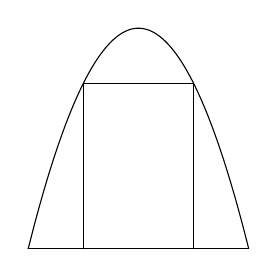
\begin{tikzpicture}[line join = round, line cap = round,>=stealth,font=\footnotesize,scale=.7,declare function={f(\x)=4-(\x)^2;}]
		\draw[samples=200,domain=-2:2,smooth] plot (\x, {f(\x)});
		\def \a{1}
		\draw (-\a,0)|-(0,{f(\a)})-|(\a,0) (-2,0)--(2,0);
		\end{tikzpicture}
	}
	\loigiai{
		\immini
		{
			Chọn hệ trục tọa độ như hình vẽ.\\
			Vì vòm hoa hình parabol nên có phương trình là $x^2=2py$.\\
			Vì căn biệt thự nhà anh $A$ có cánh cổng cao $3$ m, rộng $4$ m nên vòm hoa đi qua điểm $(2;3)$.\\
			Thay $x=2$, $y=3$ vào $x^2=2py$, ta được $p=\dfrac{2}{3}$.\\
			Vậy $x^2=\dfrac{4}{3}y$.\\
			Do vòm hoa cao $4$m nên ta có $y=4$.\\
			Thay $y=4$ vào $x^2=\dfrac{4}{3}y$, ta có $x=\pm\dfrac{4}{\sqrt{3}}$.\\
			Vậy khoảng cách giữa hai chân vòm hoa là $\dfrac{8}{\sqrt{3}}$m để đáp ứng yêu cầu của anh $A$.
		}
		{
		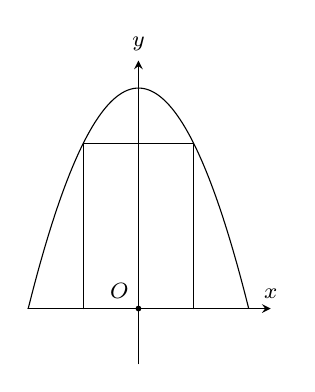
\begin{tikzpicture}[line join = round, line cap = round,>=stealth,font=\footnotesize,scale=.7,declare function={f(\x)=4-(\x)^2;}]
		\draw[samples=200,domain=-2:2,smooth] plot (\x, {f(\x)});
		\def \a{1}
		\draw (-\a,0)|-(0,{f(\a)})-|(\a,0) (-2,0)--(2,0);
		\def\xt{-2}\def\xp{2.4}\def\yd{-1}\def\yt{4.5}
		\def \a{0.7}
		\draw[->] (\xt,0)--(\xp,0) node[above]{$x$};
		\draw[->] (0,\yd)--(0,\yt) node[above]{$y$};
		\fill (0,0) circle (1.5pt) node[above left]{$O$};
		\end{tikzpicture}
		}
	}
\end{ex}